
%include diagram

High energy electrons\footnote{Throughout this section we use 
electrons to collectively refer to both electrons and positrons
unless otherwise specified.} produced from the 
hard scatter of the proton-proton
collisions of the LHC
will frequently radiate photons in the presence of the ATLAS
detector material. Furthermore, it is also common %how common?
for high energy photons to decay into an electron-positron pair.
These two processes are shown as Feynman diagrams 
separately in \fig\ref{}.
Chaining these two processes together will cause 
an electron (positron) to radiate a photon which then produces an
electron-positron pair, resulting in a three body final state with
two electrons (positrons) and a positron (electron).
Often, the energy difference between the products in the final state will
be large, such that the most of the energy is carried away in only one
product.  It is thus possible that majority of the energy of the initial
electron (positron) is carried away in the positron (electron), which
has an opposite charge.  If the energy imbalance is large enough,
the other two final state electrons (positrons) may not have enough
energy to be reconstructed. As a result, the initial electron
(positron) will instead be measured as a positron (electron), and the 
charge of initial state electron (positron) will have effectively 
been mis-identified. 


%need to do some research on bethe-bloche.
The probability of this to occur is non-negligible in the presence of the material 
from the ATLAS detector. This is due to bethe-bloche...
While muons are also technically also capable of such a phenomenon, the 
energies required are too large, according to bethe-bloche.
Indeed, we observe that the rate of charge mis-identification for muons
is vanishingly small and so we neglect it. %or should I just say that it should be?

The strong dependence upon the ATLAS material means that care must be
taken when describing this process. In particular, the material 
description in MC, while sophisticated, is not perfect. Thus, the use of MC
for determining the rate of electron charge mis-identification is inherently
flawed. Instead, it would be better to use the data itself to determine
a model for these rates. 
Thus, we extract the rates of electron charge 
mis-identificatoin using the data and only use the rates determined
in MC as a cross-check.

The background due to electron charge mis-identification is most important 
for this analysis
in the 0 SFOS signal region, described in \sec\ref{sec:signal_regions},
where it is one of the only mechanisms by which the $WZ$ and $ZZ$ 
processes enter this region\footnote{The $WZ$ and $ZZ$ processes
can also enter in the 0 SFOS region if the $Z$ bosons
decay to $\tau$ leptons which then subsequently decay into 
either electrons or muons with the proper charge and flavor combination.}.
Without electron charge mis-identification, these events would fall
equally in the 1 and 2 SFOS regions.
As will be seen shortly, the overall rate of electron charge mis-identification
is quite small (calculate???). 
Furthermore, it will be seen that the total background in the 0 SFOS region is 
a good deal smaller than the the 1 and 2 SFOS regions. Thus, the
migration of events from the 1 and 2 SFOS regions to the 0 SFOS 
region, resulting from electron charge mis-identification, has
a larger relative impact on the background in the 0 SFOS 
region\footnote{There is also a migration from the 0 SFOS to the 1 and 2 SFOS 
regions, but the relative number of 0 SFOS events to 1 and 2 SFOS
events before electron mis-identification is so small as to make this
effect completely negligible.}.
As a result, we focus only on modelling the background due to electron
charge mis-identification in the 0 SFOS region and assume that an 
out of the box estimate of this background from MC is adequate for the 
1 and 2 SFOS regions.


The electron charge mis-identification background is determined
for the 0 SFOS signal region by first extracting the electron charge
mis-identification rates using the data as a model
described below. The extracted
rates are compared to an alternative method using only MC. 
The difference between the two is used as a systematic on the
rates. The rates are then used to reweight the $WZ$ and $ZZ$ MC samples
on an event-by-event basis 
according to the probability that electron charge mis-identification
could cause the event to migrate into the 0 SFOS region. In this way, 
the full statistics of the MC samples can be utilitized to get a model of
the behvaior of these processes in the 0 SFOS region, while also taking 
into account a more accurate material description. Other backgrounds
due to electron charge mis-identification are assumed to be negligible.
More details on the methods used to extract the rates and the re-weighting
method are provided below.




\subsubsection{Charge Mis-identification Rate Extraction}

The rate of electron charge mis-identification is defined as 
the probability that an electron has it's charge mis-identified.
These rates depend highly on the kinematics of the individual electrons.
In particular, the sensitivity to material dependence described above 
means that the rate depends on where in the detector the electrons
pass through. In general, the material density of the ATLAS
detector increases for high \eta~(i.e. as the electron gets closer to the
beam pipe). The rate also increases as a function of the electron energy, 
or \pt. These are the two most important kinematic variables for determining
the rate\footnote{The material also varies as a function of the azimuthal angle,
$\phi$, in the detector. However, this is a sub-dominant effect. Furthermore,
increasing the dimensionality further significantly harms the statistical 
power of the method. Thus it is ignored.}, and 
so the rate extraction is binned as a function of both with nine $\eta$ 
bins ranging from 0 to 2.5 and six \pt~bins ranging from 15 to 120 \GeV~plus
an additional overflow bin for $\pt>120\GeV$.



The rates are studied in a region with two electrons passing the object
selection from \sec\ref{sec:www_object_selection} and that have
a di-lepton mass within 10~\GeV of the \z mass. No requirements are placed
on their charge. Two different methods
are used: one using purely MC and one using the data.
The method using MC takes $\z\rightarrow ee$ MC simulation 
and relies on being able to determine the charge of each electron from the 
\z decay by looking 
directly from at hard scattering process as provided by the generator.
This is called ``truth'' information, at which point the processes of radiation
and pair-production have not occured. It then compares
these truth electrons to the reconstructed electrons 
measured after all processes, including those of radiation and pair-production,
have been simulated and have been reconstructed
in the detector. The truth electrons and reconstructed electrons
are matched by asking that they are nearby eachother in $\eta$ and $\phi$.
The charge of the matched truth and reconstruction electrons 
are then compared and it is recorded whether or not the charges agree
in the appropriate $\pt$ and $\eta$ bin. Once all MC events
have been recorded, the rate per bin may be determined simply 
by taking the ratio of the number of electrons where the truth and reconstructed
electron charge disagreed per bin to the total number of electrons per bin. 

The nominal method for extracting the electron charge mis-identification
rates is instead one that uses the data exclusively. 
It uses the same selection as in the MC method, with the events
categorized based on whether the electrons from the \z
decay are of the same-sign or of opposite-sign.
However, in this case
there is no truth information to tell which electron's charge
has been mis-identified. Instead, we assume that those events in
the same-sign cateogry are due purely to charge mis-identification
and attempt to extract the rates by minimizing a likelihood.
Refer to the rate for an electron in a 
particular $\pt$ and $\eta$ bin $i$ as $\varepsilon_i$.
Also, refer to the total number of events observed in data with one electron
in bin $i$ and the other in bin $j$ as $N_{i,j}$.
Given the rates, the expected number of same-sign events
should be approximately $N_{i,j}(\varepsilon_i + \varepsilon_j)$,
where we have ignored the probability for both electrons to have their
charges flipped since it should be small. We do
not know the rates \emph{a priori}, but they should follow 
a Poisson likelihood given the observed total number of events,
$N_{i,j}$, and the the observed number of same sign events,
$N_{i,j}^{\textrm{SS}}$, with the following form:
\begin{equation}
\curlyl( \varepsilon_i,\varepsilon_j | N_{i,j}^{\textrm{SS}},N_{i,j})
=
\frac{(N_{i,j}(\varepsilon_i+\varepsilon_j))^{N^{\textrm{SS}}_{i,j}} e^{-N_{i,j}(\varepsilon_i+\varepsilon_j)}}{N^{\textrm{SS}}_{i,j}!}
\end{equation}
From this, we may construct a log likelihood which can be minimized
as a function of $\varepsilon_i$ and $\varepsilon_j$:
\begin{equation}
-\ln \curlyl( \varepsilon_i,\varepsilon_j | N_{i,j}^{\textrm{SS}},N_{i,j}) = 
N_{i,j}(\varepsilon_i+\varepsilon_j)
- N^{\textrm{SS}}_{i,j} \ln(N_{i,j}(\varepsilon_i+\varepsilon_j))
\end{equation}
where the terms that are not dependent on $\varepsilon_i$
and $\varepsilon_j$ have been dropped.
Thus, given the data, the values of $\varepsilon_i$ and $\varepsilon_j$
at the minimum value of the log likelihood are taken as the estimate
of the rates.

The rates for the two different methods are shown in \fig\ref{}.
%these should be contour maps.
The behavior is as follows... 


The rates are also determined after subtracting the background. 
This is done by....

The different rate estimations are summarized in \fig\ref{}.
%big summary table.
The systematics on the rates are determined by...

\subsubsection{Di-boson MC Reweighting with Rates}

We reweight the MC in the 0 SFOS region to extract an estimate

\subsubsection{Validation}


\subsubsection{Comparison between Likelihood rate and Truth rate}
   The mis-charge rate for $Z\rightarrow ee$ MC sample is measured
   using the likelihood method and is compared with truth mischarge
   rate in Fig.~\ref{fig:LL_Truth_Comparison}.

\begin{figure}[htp]
\centering
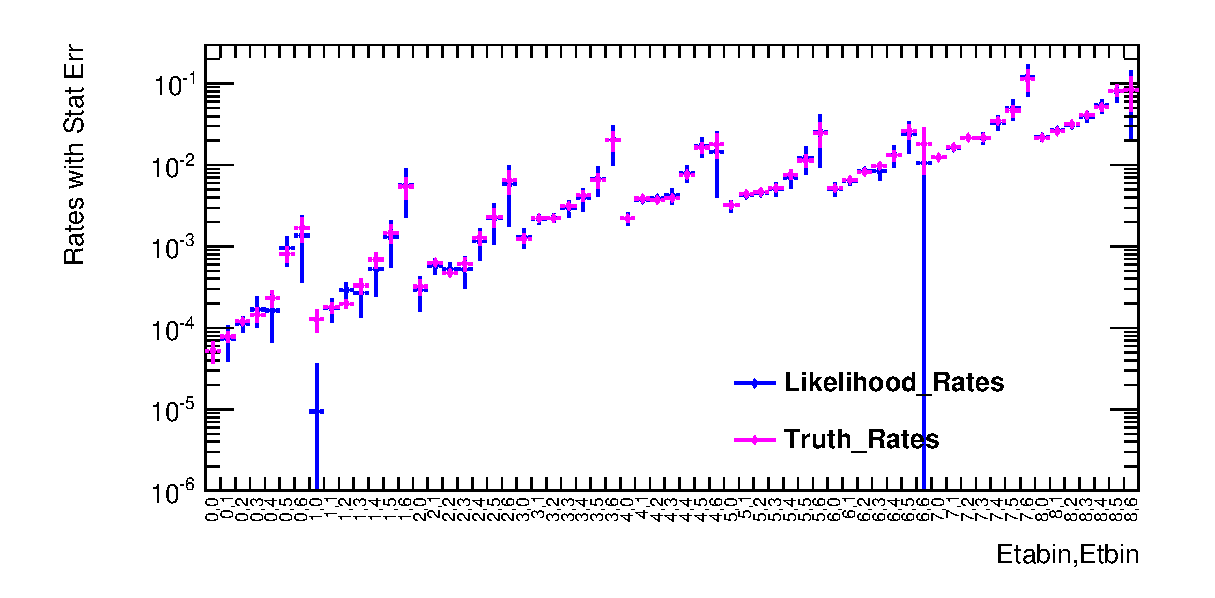
\includegraphics[width=0.8\textwidth]{figures/ChargeMisID/LL_TR_Com.eps}
\caption{This is mis-charge rate comparison between likelihood and
  truth method considering statistic errors. The two sets of rates
  here are both measured with \Zee\ MC samples. The $x$ axis label is
  the \eta, \pt\ bin index.}
\label{fig:LL_Truth_Comparison}
\end{figure}  

Through the comparison, we can see that the rates measured with
likelihood method are compatible with what we measured with truth
method. Using the likelihood method, we measure the mischarge rate
with real data in Egamma stream we measure the data-driven rates with
Egamma
samples(\texttt{user.along528.data12\_8TeV.period*.physics\_EGamma.PhysCont.NTUP\_SMWWW.SMN2N\_2\\Lep\_v1\_EXT0}
where * is A,B,C,D,E,G,H,I,J,L. These samples are slimmed with loose
di-lepton requirement, the di-lepton slim require there are at least 2
tagged high \pt\ leptons where tagged high \pt\ means Electron/Muon
satisfies any object quality requirement (loose, medium or tight for
muons and loose++,\\medium++,tight++,
veryLooseLL,looseLL,mediumLL,tightLL, or veryTightLL for electrons)
and has a pt of at least 10 GeV.). We use the data-driven likelihood
rates as our central values with the effect of background
contamination neglected. We estimate the background effect with
coarser binning and include the shift in mischarge rate in the
systematics.

%  We apply the likelihood method and event selection mentioned before
%  to data and we get the data-driven electron mis-charge rates, but
%  the rates are measured from data so there will be background events
%  remaining in the selected events. We use those rates directly
%  measured from data as central values and then subtract the
%  background contribution in the rates, we can calculate another set
%  of likelihood rates using the events without background, we may
%  call those rates clean rates. The difference between central values
%  and clean rates is the background systematic.

\begin{figure}[htp]
\centering
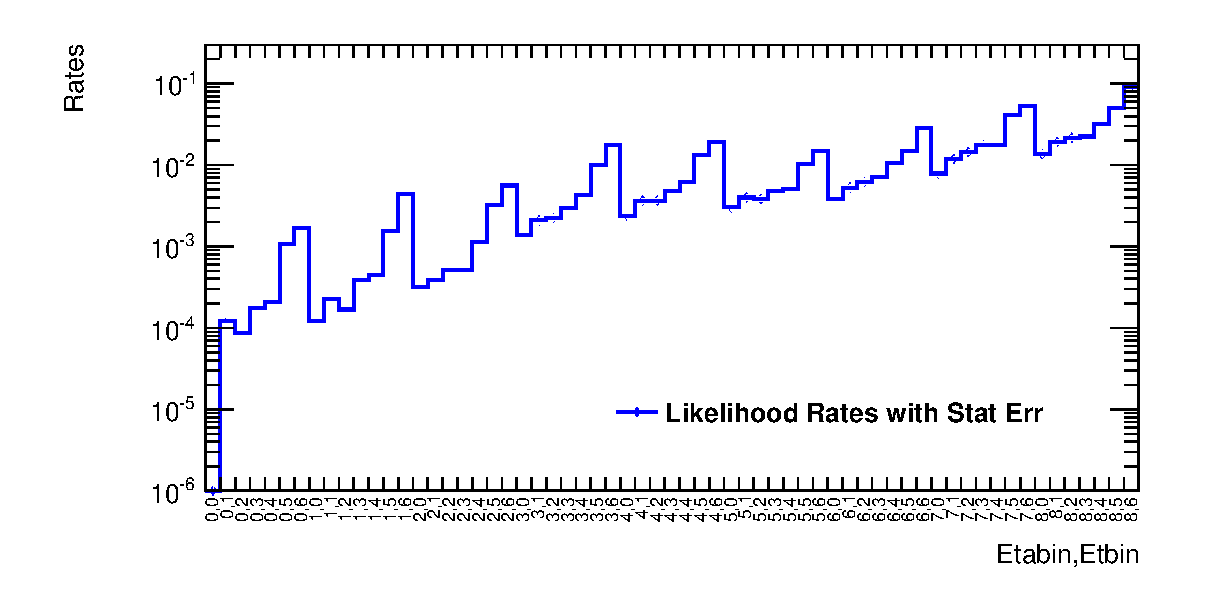
\includegraphics[width=0.8\textwidth]{figures/ChargeMisID/Egamma_LL.eps}
\caption{This is electron mis-charge rates measured from data with likelihood method and its statistic errors. Label on x axis is \eta, \pt\ bin indices.}
\label{fig:LL_Rates_Egamma}
\end{figure}

We use template fit method on the distribution of invariant mass of
the electron pairs to determine the background contribution in total
number of events in each bin ($N^{i,j}_{tot}$ in
Eq.~(\ref{eq:lnL_chargeMisID})) and in number of same sign events in each
bin ($N^{i,j}_{SS}$ in Eq.~(\ref{eq:lnL_chargeMisID})).  We subtract the
estimated background contribution in $N^{i,j}_{SS}$ and
$N^{i,j}_{tot}$ before maximizing the likelihood. This is only
practical with much coarser bins. The signal template is obtained from
\Zee\ MC, and the background template is obtained with data, with some
electron identification and isolation cuts reversed.

\begin{table}
  \centering
  \begin{tabular}{|c|c|}
  \hline
  Signal & Background \\
  \hline
  \texttt{EF\_e24vhi\_medium1} or \texttt{EF\_e60\_medium1} & \texttt{EF\_e24vhi\_medium1} or \texttt{EF\_e60\_medium1} \\
  \hline
  Exactly two electrons passing electron selection & Choose the leading and sub-leading electrons \\ & and at least one of these 2 electrons \\ & satisfied the background electron selection \\
  \hline
  Trigger Match & \\
  \hline
  $|$ee Invariant Mass - Zmass$|$$\textless$10 GeV & \\
  \hline
  \end{tabular}
\caption{Event selection to select signal and background $ee$ invariant mass histograms.}
\label{tab:Event_Selection}
\end{table}

\begin{table}
  \centering
  \begin{tabular} {|c|c|}
  \hline
  Signal  & Background \\
  \hline
  Author is 1 or 3 & Author is 1 or 3 \\
  \hline
  OQ & OQ \\
  \hline
  $|$\eta$|$ $\textless$ 2.47, crack region removed & $|$\eta$|$ $\textless$ 2.47, crack region removed \\
  \hline
  \pt\ $\textgreater$ 15 GeV & \pt\ $\textgreater$ 15 GeV \\
  \hline
  TightPP & fail TightPP \\
  \hline
  ETcone20/\pt\ $\textless$ 0.10 for \pt\ $\textgreater$ 20GeV & Fail this cut\\ ETcone20/\pt\ $\textless$ 0.07 for \pt\ $\textless$ 20GeV & \\
  \hline
  pTcone20/\pt\ $\textless$ 0.04 & Fail this cut \\
  \hline
  $|$d0/sigmad0$|$$\textless$3.0 & \\
  \hline
  $|$z0*sin(theta)$|$$\textgreater$0.5 & \\
  \hline
  \end{tabular} 
\caption{Electron selection to select signal and background ee
  invariant mass histograms.}
\label{tab:Electron_Selection}
\end{table}

%  With the event and electron selection we can get the signal $ee$ invariant mass histogram from \Zee\ MC samples and background $ee$ invariant mass histogram from data. Because the events are divided into many bins and the statistic will be too low to apply template fit, we will merge the bins of the electrons so that we will get enough statistic to do background subtraction. 
To improve the statistical precision, we merge the $p_T$ bins and then
the events will be divided into $9\times 9$ \eta-bins. We will choose
events with the first electron's $|\eta|$ between [0,0.8] and the
second electron's $|\eta|$ between [1.15,1.60] to illustrate the
procedure. The $ee$ invariant mass distribution obtained from the
\Zee\ MC samples using the background selection (shown in
Table~\ref{tab:Electron_Selection}) is presented in
Fig.~\ref{fig:Mee} (left) and the background $ee$ invariant mass
selected from data using the background selection is presented in
Fig.~\ref{fig:Mee} (right).
 
\begin{figure}[htbp] 
  \centering
  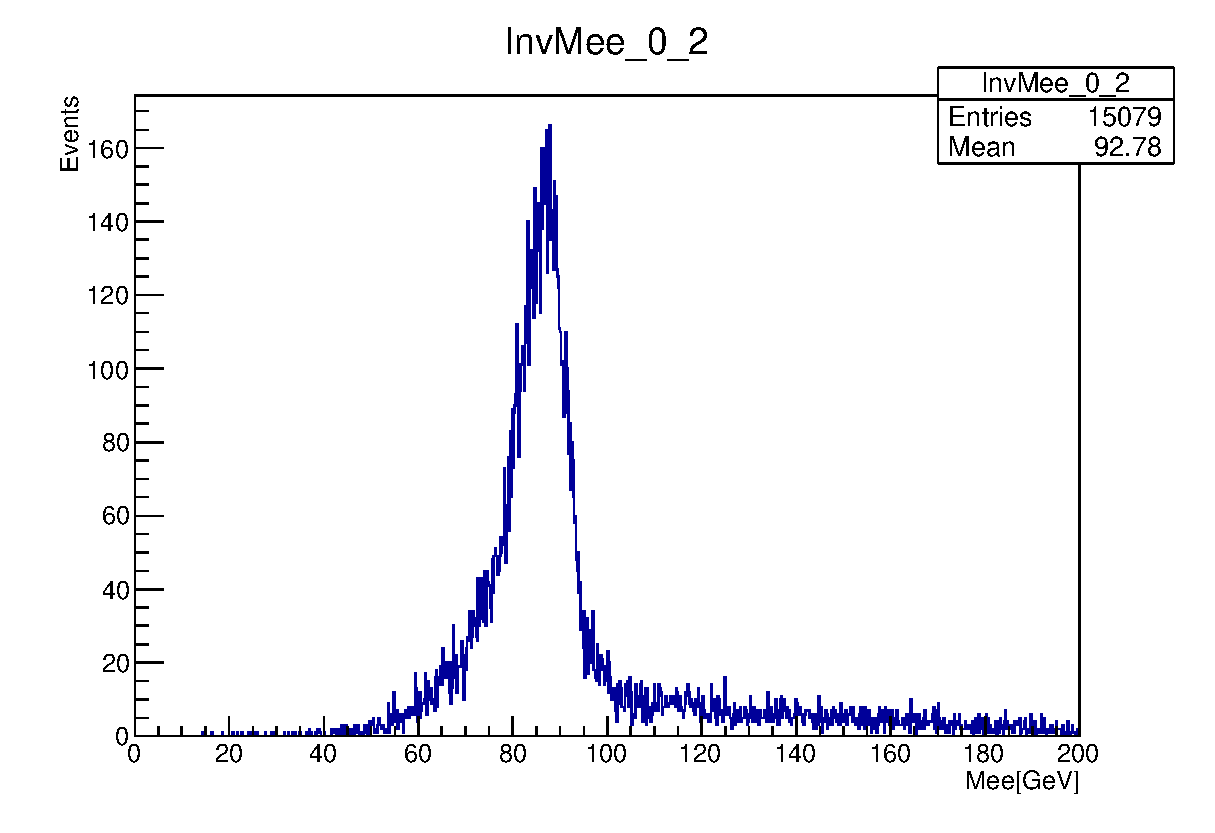
\includegraphics[width=0.49\textwidth]{figures/ChargeMisID/MergeEt_Ntot_ZeeBkg02.eps}
  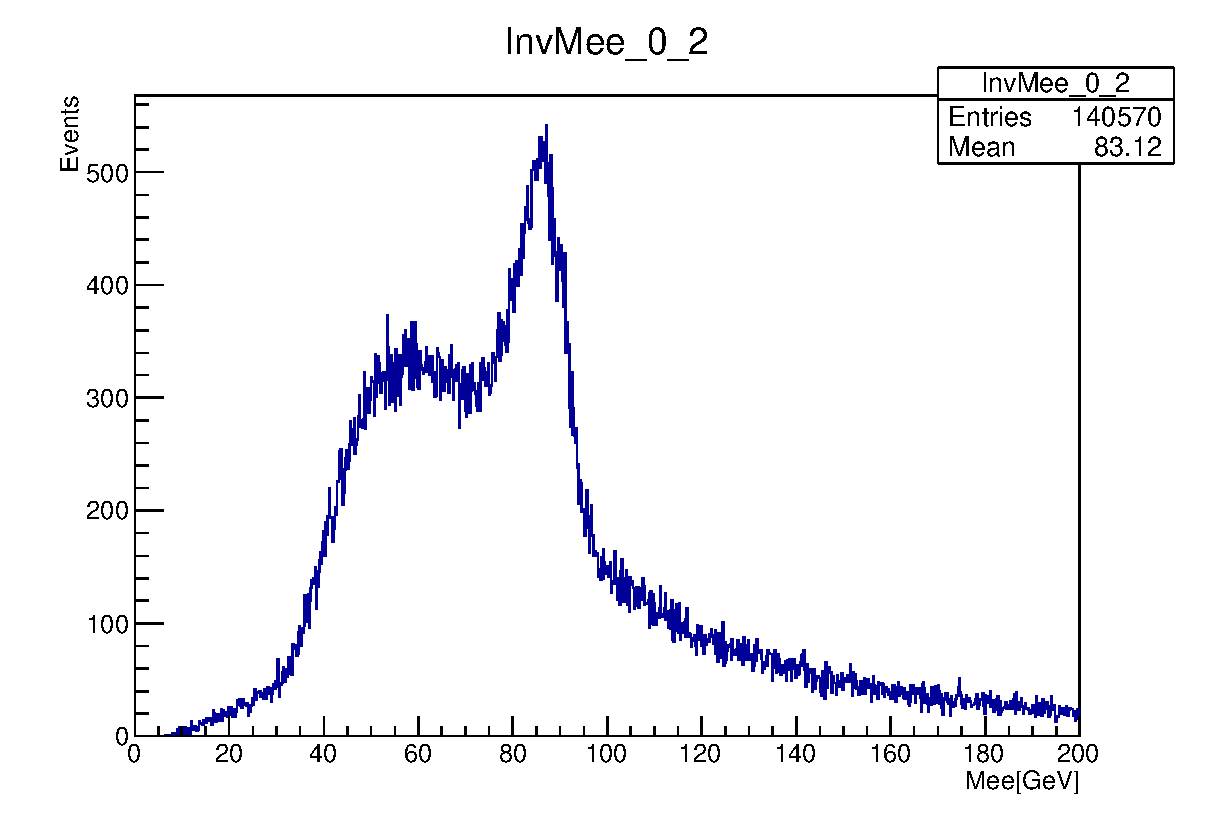
\includegraphics[width=0.49\textwidth]{figures/ChargeMisID/MergeEt_Ntot_Bkg02.eps}
  \caption{The $ee$ invariant mass obtained from \Zee\ MC samples
    (left) and from data (right) using the background selection in
    Table~\ref{tab:Electron_Selection} and
    Table~\ref{tab:Event_Selection}.}
  \label{fig:Mee}
\end{figure}

 We can see that the signal $ee$ invariant mass histogram looks fine
 but for the background $ee$ invariant mass histogram, there is an
 obvious peak around $Z$ mass area which is because there are
 \Zee\ events remaining in the background histogram. We fit the $ee$
 invariant mass spectrum with signal template obtained from MC and a
 polynomial function to describe the background. The polynomial
 function obtained in the fit is then used as the background
 template. The polynomial fit for events with first electron's
 $|\eta|$ between [0,0.8] and second electron's $|\eta|$ between
 [1.15,1.60] is shown in Fig.~\ref{fig:Polynomialac}.
\begin{figure}[htp]
\centering
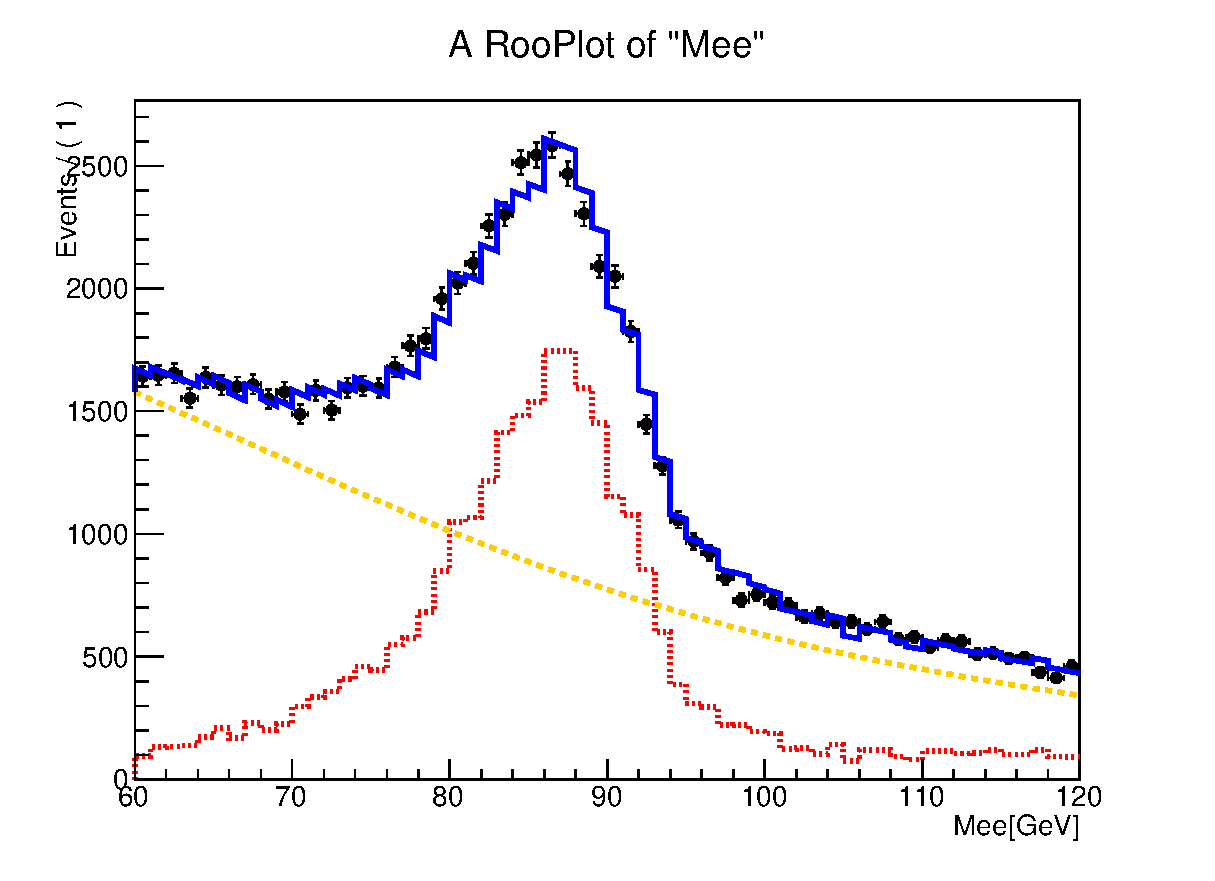
\includegraphics[width=0.5\textwidth]{figures/ChargeMisID/Tot_Polynomial_0_2.eps}
\caption{This plot is polynomial fit for events with first electron's
  $|\eta|$ between [0,0.8] and second electron's $|\eta|$ between
  [1.15,1.60], red line is the \Zee\ signal component, orange
  polynomial is the background component from the fit, black solid
  line is from data sample selected using reversed electron
  identification and isolation cuts and the blue line is the fit.}
\label{fig:Polynomialac}
\end{figure} 

%From Figure.~\ref{fig:Polynomialac}, we can see that the polynomial fit is successful and in this way we can get clean background $ee$ invariant mass histograms for different bins and we use the 4th order polynomial functions obtained here as background templates. 
Thus we can use template fit to estimate the amount of background in
data with the signal template and background template. The signal
template is shown in Fig.~\ref{fig:Signal} and the template fit for
events whose first electron's $|\eta|$ between [0,0.8] and second
electron's $|\eta|$ between [1.15,1.60] is presented in
Fig.~\ref{fig:Template fit}.
\begin{figure}[htp]
  \begin{minipage}[t]{0.5\linewidth}
  \centering
  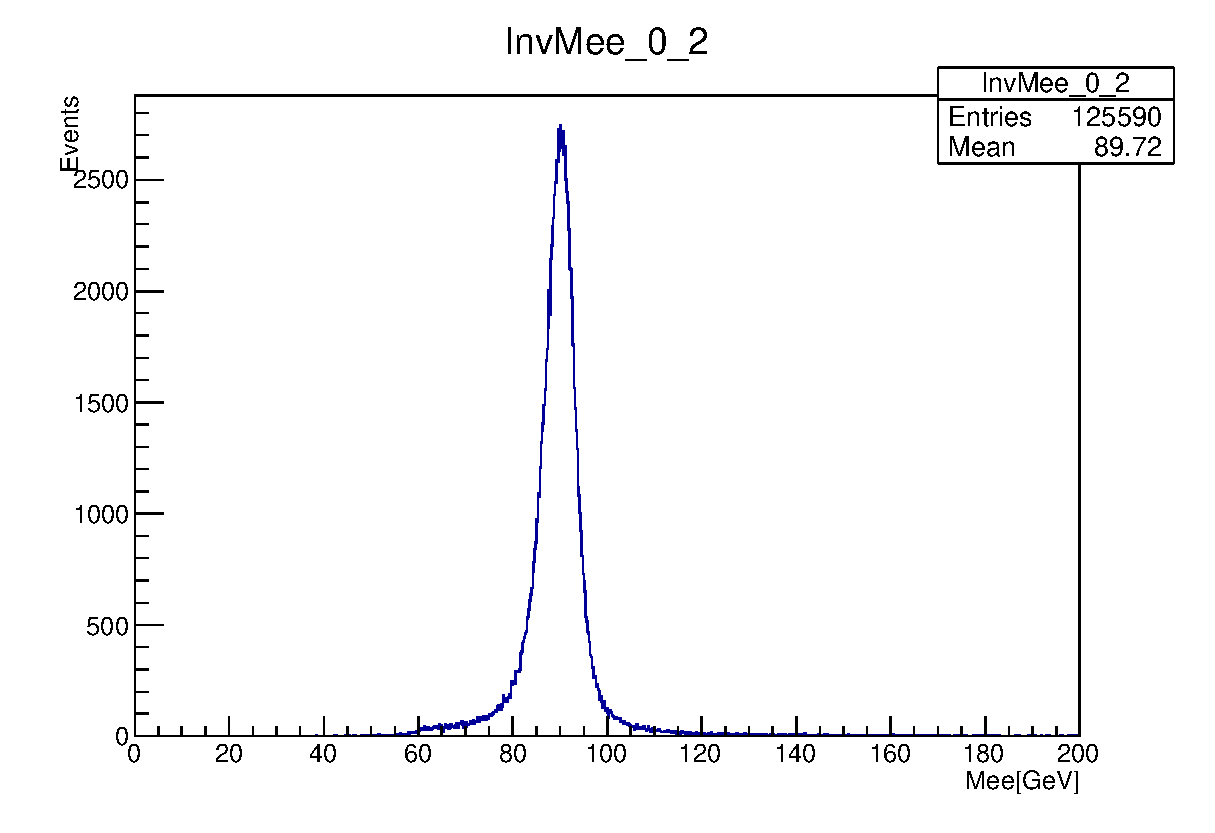
\includegraphics[width=\columnwidth]{figures/ChargeMisID/MergeEt_Ntot_Zee02.eps}
  \caption{Signal $ee$ invariant mass distribution}
  \label{fig:Signal}
  \end{minipage}
  \begin{minipage}[t]{0.5\linewidth}
  \centering
  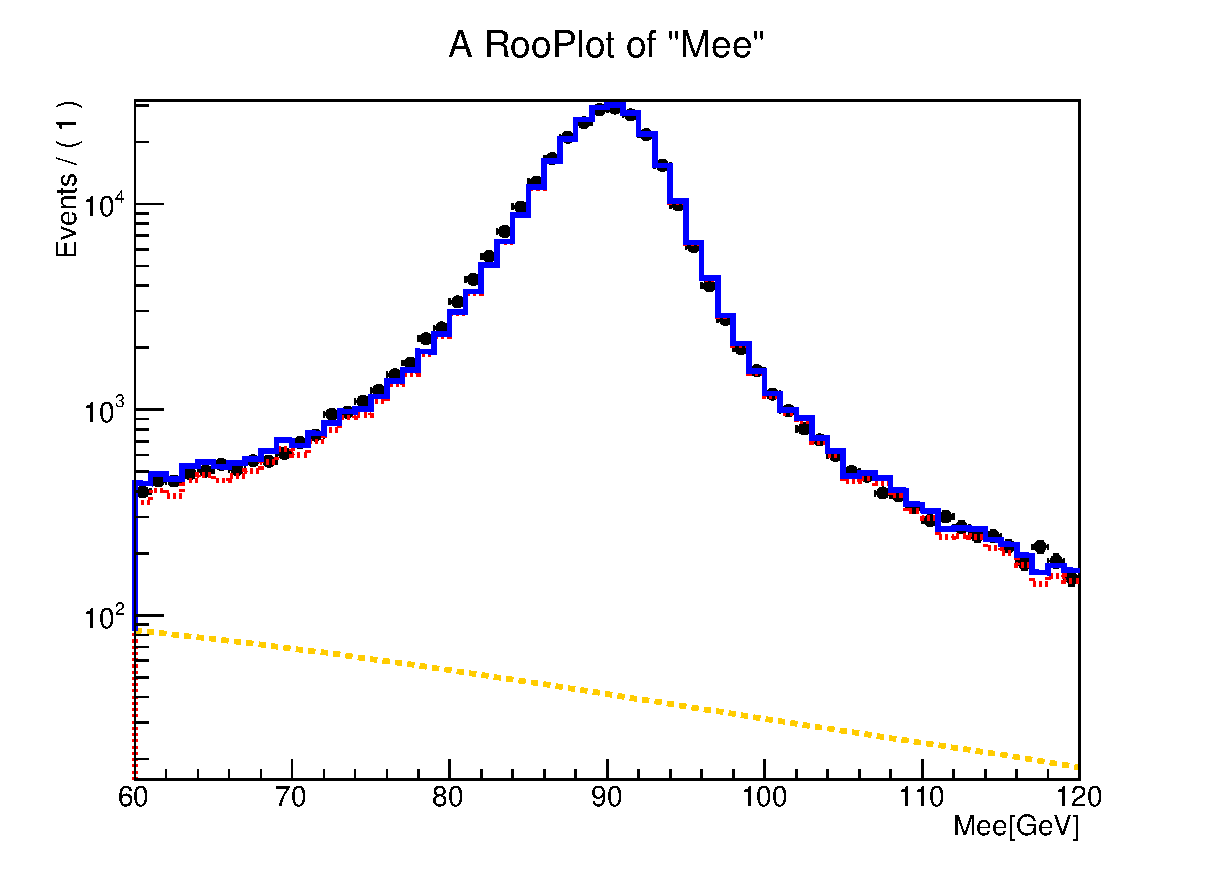
\includegraphics[width=\columnwidth]{figures/ChargeMisID/Tot_Template_0_2.eps}
  \caption{This plot is template fit for events with first electron's $|\eta|$ between[0,0.8] and second electron's $|\eta|$ between[1.15,1.60], red line is the \Zee\ signal component, orange polynomial is the background component from the fit, black solid line is from data sample and the blue line is the fit.}
  \label{fig:Template fit}
  \end{minipage}
\end{figure}  

With template fit, we can get the signal purities in different bins, and we use the signal purities here to estimate the background amount. We need the signal purity of both total events and same sign events to calculate another set of mis-charge rates without background contamination. The numbers presented in Table~\ref{tab:fSig Ntot} and Table~\ref{tab:fSig error Ntot} are the signal purity and statistic errors of signal purities for total events. 
\begin{table}
\footnotesize
\centering
\begin{tabular}{c|c|c|c|c|c|c|c|c|c}
  \hline
   &[0,0.8] &[0.8,1.15] &[1.15,1.60] &[1.60,1.80] &[1.80,2.0] &[2.0,2.20] &[2.20,2.30] &[2.30,2.40] &[2.40,2.50] \\
  \hline
  [0,0.8]  &0.9951 &0.9966 &0.9945 &0.9956 &0.9953 &0.9924 &0.9961 &0.9898 &0.9893 \\
  \hline
  [0.8,1.15]  &0.996 &0.9982 &0.9933 &0.9887 &0.9939 &0.9953 &0.992 &0.9935 &0.972 \\
  \hline
  [1.15,1.60]  &0.9904 &0.9895 &0.9892 &0.9885 &0.9895 &0.9942 &0.9875 &0.9912 &0.9802 \\
  \hline
  [1.60,1.80] &0.9794 &0.9766 &0.9787 &0.9799 &0.9828 &0.9822 &0.9775 &0.9674 &0.9534 \\
  \hline
  [1.80,2.0]  &0.9914 &0.992 &0.994 &0.9878 &0.9927 &0.9906 &0.9906 &0.9912 &0.9546 \\
  \hline
  [2.0,2.20] &0.9934 &0.9978 &0.9833 &0.9872 &0.9936 &0.9847 &0.9837 &0.9717 &0.9776 \\
  \hline
  [2.20,2.30] &0.998 &0.9874 &0.9901 &0.9743 &0.992 &0.9874 &0.9813 &0.9835 &0.9509 \\
  \hline
  [2.30,2.40] &0.9891 &0.9883 &0.9825 &0.9734 &0.9916 &0.9846 &0.9698 &0.9643 &0.9739 \\
  \hline
  [2.40,2.50] &0.9774 &0.9636 &0.9794 &0.9703 &0.9766 &0.9805 &0.9804 &0.9509 &0.9211 \\
  \hline
\end{tabular}
\caption{Signal purity for total events, different rows stand for different $|\eta|$ bins of the sub-leading electron in the event, and different columns stand for different $|\eta|$ bins of the leading electrons in the event.} 
\label{tab:fSig Ntot}
\end{table}
 
\begin{table}
\footnotesize
\centering
\begin{tabular}{c|c|c|c|c|c|c|c|c|c}
  \hline
   &[0,0.8] &[0.8,1.15] &[1.15,1.60] &[1.60,1.80] &[1.80,2.0] &[2.0,2.20] &[2.20,2.30] &[2.30,2.40] &[2.40,2.50] \\
  \hline
  [0,0.8] &0.0004 &0.0006 &0.0008 &0.0011 &0.0012 &0.0011 &0.0016 &0.0019 &0.0028\\
  \hline
  [0.8,1.15] &0.0006 &0.0010 &0.0013 &0.0020 &0.0021 &0.0019 &0.0029 &0.0030 &0.0038 \\
  \hline
  [1.15,1.60] &0.0008 &0.0013 &0.0016 &0.0023 &0.0021 &0.0020 &0.0027 &0.0031 &0.0038 \\
  \hline
  [1.60,1.80] &0.0013 &0.0021 &0.0022 &0.0030 &0.0027 &0.0027 &0.0036 &0.0043 &0.0058 \\
  \hline
  [1.80,2.0] &0.0012 &0.0019 &0.0021 &0.0026 &0.0025 &0.0022 &0.0024 &0.0044 &0.0055 \\
  \hline
  [2.0,2.20] &0.0013 &0.0016 &0.0021 &0.0024 &0.0025 &0.0023 &0.0035 &0.0035 &0.0051 \\
  \hline
  [2.20,2.30] &0.0017 &0.0029 &0.0029 &0.0037 &0.0045 &0.0029 &0.0058 &0.0044 &0.0076 \\
  \hline
  [2.30,2.40] &0.0019 &0.0030 &0.0032 &0.0039 &0.0031 &0.0029 &0.0045 &0.0046 &0.0061 \\
  \hline
  [2.40,2.50] &0.0031 &0.0048 &0.0045 &0.0051 &0.0046 &0.0040 &0.0061 &0.0072 &0.0118 \\
  \hline
\end{tabular}
\caption{Statistical uncertainties of the purities listed in Table~\ref{tab:fSig Ntot}}
\label{tab:fSig error Ntot}
\end{table}

For the same-sign events, the same method is used to estimate the
background contribution, but with all events merged because the
statistics is very limited in the data sample. The global polynomial
fit for same sign events is shown in Fig.~\ref{fig:Global Polynomial}
and the global template fit for same sign events is shown in
Fig.~\ref{fig:Global Template}.
\begin{figure}[htp]
  \begin{minipage}[t]{0.5\linewidth}
  \centering
  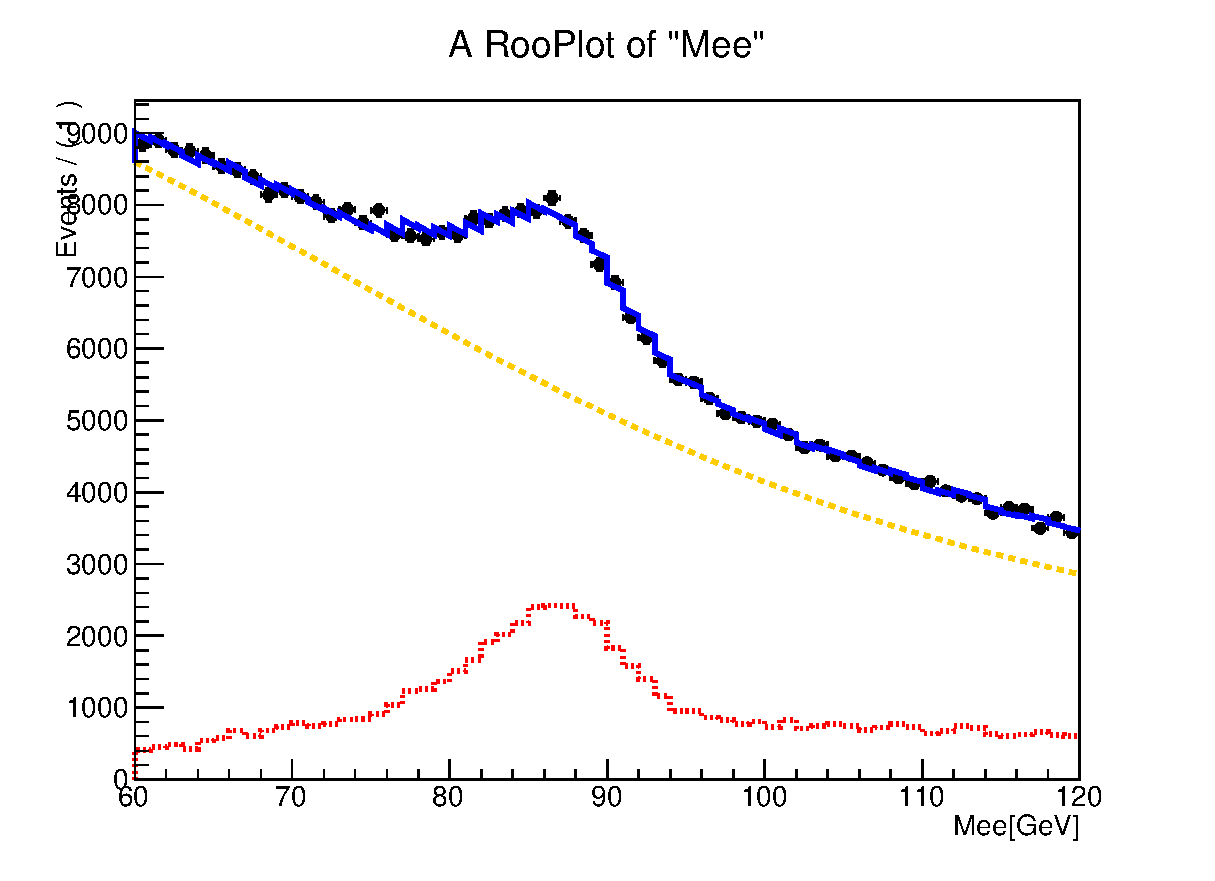
\includegraphics[width=\columnwidth]{figures/ChargeMisID/SS_Polynomial.eps}
  \caption{Global polynomial fit for total events}
  \label{fig:Global Polynomial}
  \end{minipage}
  \begin{minipage}[t]{0.5\linewidth}
  \centering
  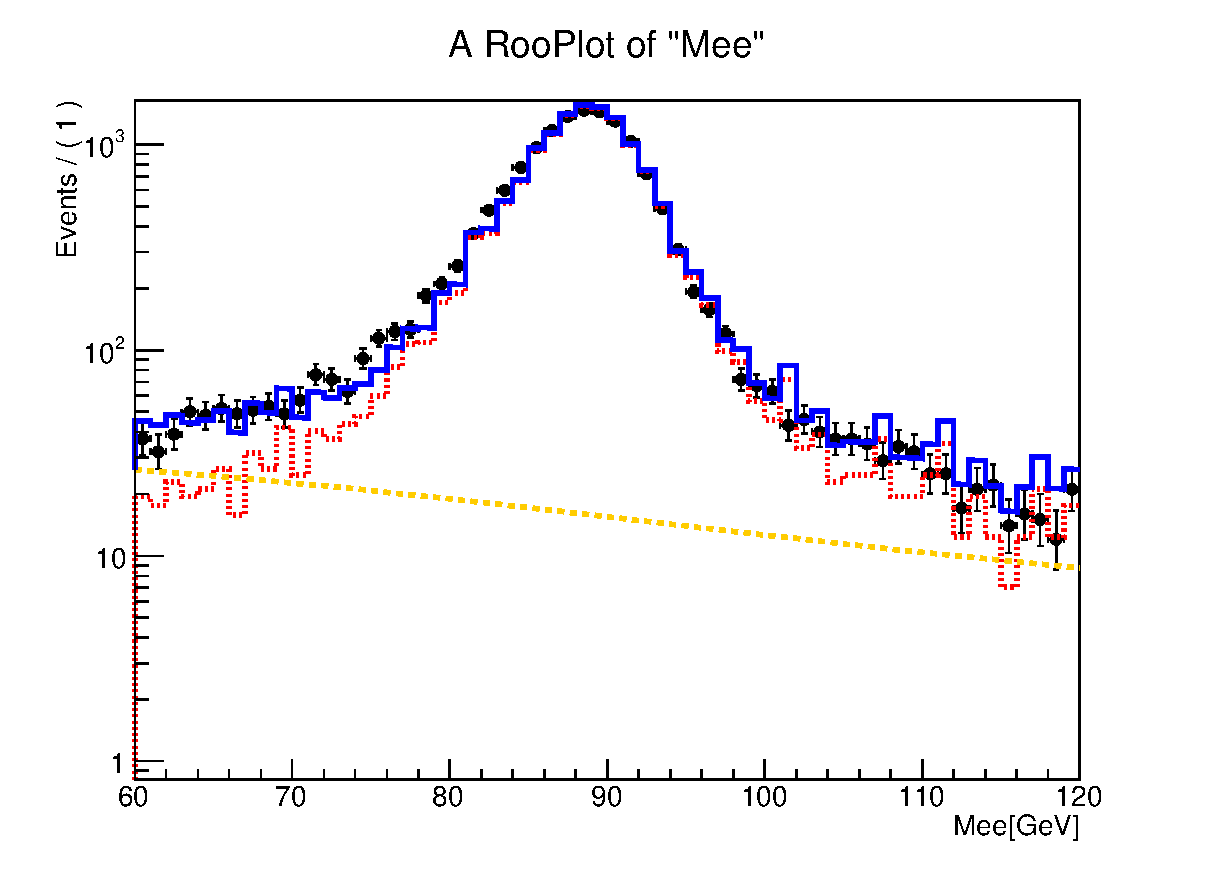
\includegraphics[width=\columnwidth]{figures/ChargeMisID/SS_Template.eps}
  \caption{Global template fit for same sign events.}
  \label{fig:Global Template}
  \end{minipage}
\end{figure} 

Using the template fitting, we obtain the global purity of same sign
events as 0.9372$\pm$0.0042(stat), and the global purity of opposite
sign events as 0.9921$\pm$ 0.0013(stat). The ratio of signal purities
is 0.9447 and is assumed to be independent of different $\eta$
bins. For each $\eta_1 - \eta_2$ bin, we scale the purity of opposite
sign events with this ratio to obtain an estimation of the purity of
the same sign events.

\begin{table}
\footnotesize
\centering
\begin{tabular}{c|c|c|c|c|c|c|c|c|c}
  \hline
   &[0,0.8] &[0.8,1.15] &[1.15,1.60] &[1.60,1.80] &[1.80,2.0] &[2.0,2.20] &[2.20,2.30] &[2.30,2.40] &[2.40,2.50] \\
  \hline
  [0,0.8] &0.9958 &0.997 &0.9947 &0.9958 &0.9951 &0.9924 &0.9968 &0.9871 &0.9863 \\
  \hline
  [0.8,1.15] &0.9964 &0.9982 &0.9937 &0.9882 &0.9937 &0.9951 &0.9924 &0.993 &0.9707 \\
  \hline
  [1.15,1.60] &0.9904 &0.9896 &0.9889 &0.9883 &0.9899 &0.9938 &0.988 &0.9913 &0.9792 \\
  \hline
  [1.60,1.80] &0.9786 &0.9765 &0.9784 &0.9771 &0.9811 &0.9815 &0.9753 &0.9638 &0.9483 \\
  \hline
  [1.80,2.0] &0.9907 &0.9918 &0.9944 &0.9876 &0.9921 &0.9911 &0.9893 &0.9924 &0.9527 \\
  \hline
  [2.0,2.20] &0.9938 &0.9979 &0.9826 &0.9882 &0.9934 &0.9815 &0.9844 &0.9735 &0.9777 \\
  \hline
  [2.20,2.30] &0.9982 &0.9872 &0.9903 &0.9711 &0.9921 &0.987 &0.9841 &0.9779 &0.9391 \\
  \hline
  [2.30,2.40] &0.9898 &0.9848 &0.9826 &0.9719 &0.9897 &0.984 &0.9667 &0.9562 &0.9637 \\
  \hline
  [2.40,2.50] &0.9775 &0.9656 &0.9784 &0.9628 &0.974 &0.9783 &0.9771 &0.9513 &0.9226 \\
  \hline
\end{tabular}
\caption{Signal purity of opposite sign events, different rows stand
  for different $|\eta|$ bins of the sub-leading electron in the
  event, and different columns stand for different $|\eta|$ bins of
  the leading electrons in the event.}
\label{tab:fSig Nos}
\end{table}

\begin{table}
\footnotesize
\centering
\begin{tabular}{c|c|c|c|c|c|c|c|c|c}
  \hline
   &[0,0.8] &[0.8,1.15] &[1.15,1.60] &[1.60,1.80] &[1.80,2.0] &[2.0,2.20] &[2.20,2.30] &[2.30,2.40] &[2.40,2.50] \\
  \hline
  [0,0.8] &0.0003 &0.0006 &0.0008 &0.0011 &0.0013 &0.0012 &0.0017 &0.0022 &0.0032 \\
  \hline
  [0.8,1.15] &0.0006 &0.0010 &0.0013 &0.0020 &0.0021 &0.0018 &0.0029 &0.0032 &0.0039 \\
  \hline
  [1.15,1.60] &0.0008 &0.0014 &0.0016 &0.0023 &0.0021 &0.0020 &0.0028 &0.0032 &0.0040 \\
  \hline
  [1.60,1.80] &0.0013 &0.0021 &0.0022 &0.0031 &0.0029 &0.0027 &0.0042 &0.0047 &0.0063 \\
  \hline
  [1.80,2.0] &0.0012 &0.0020 &0.0022 &0.0027 &0.0026 &0.0023 &0.0028 &0.0044 &0.0057 \\
  \hline
  [2.0,2.20] &0.0012 &0.0020 &0.0021 &0.0022 &0.0026 &0.0031 &0.0034 &0.0035 &0.0055 \\
  \hline
  [2.20,2.30] &0.0017 &0.0030 &0.0030 &0.0040 &0.0045 &0.0031 &0.0058 &0.0048 &0.0075 \\
  \hline
  [2.30,2.40] &0.0020 &0.0027 &0.0032 &0.0041 &0.0033 &0.0029 &0.0050 &0.0052 &0.0069 \\
  \hline
  [2.40,2.50] &0.0031 &0.0048 &0.0045 &0.0053 &0.0050 &0.0044 &0.0065 &0.0074 &0.0122 \\
  \hline
\end{tabular}
\caption{Statistical uncertainties of the purities listed in
  Table~\ref{tab:fSig Nos}.}
\label{tab:fSig error Nos}
\end{table}

\begin{table}
\footnotesize
\centering
\begin{tabular}{c|c|c|c|c|c|c|c|c|c}
  \hline
   &[0,0.8] &[0.8,1.15] &[1.15,1.60] &[1.60,1.80] &[1.80,2.0] &[2.0,2.20] &[2.20,2.30] &[2.30,2.40] &[2.40,2.50] \\
  \hline
  [0,0.8] &0.9407 &0.9419 &0.9397 &0.9408 &0.9401 &0.9375 &0.9417 &0.9325 &0.9317 \\
  \hline
  [0.8,1.15] &0.9413 &0.943 &0.9387 &0.9335 &0.9387 &0.9401 &0.9375 &0.9381 &0.917 \\
  \hline
  [1.15,1.60] &0.9357 &0.9349 &0.9342 &0.9337 &0.9352 &0.9389 &0.9334 &0.9365 &0.9251 \\
  \hline
  [1.60,1.80] &0.9245 &0.9225 &0.9243 &0.9231 &0.9268 &0.9272 &0.9214 &0.9105 &0.8958 \\
  \hline
  [1.80,2.0] &0.9359 &0.937 &0.9394 &0.933 &0.9372 &0.9363 &0.9346 &0.9375 &0.9 \\
  \hline
  [2.0,2.20] &0.9389 &0.9427 &0.9283 &0.9336 &0.9384 &0.9273 &0.93 &0.9197 &0.9237 \\
  \hline
  [2.20,2.30] &0.943 &0.9326 &0.9355 &0.9174 &0.9372 &0.9325 &0.9297 &0.9238 &0.8872 \\
  \hline
  [2.30,2.40] &0.935 &0.9304 &0.9283 &0.9181 &0.935 &0.9296 &0.9133 &0.9033 &0.9104 \\
  \hline
  [2.40,2.50] &0.9235 &0.9122 &0.9243 &0.9095 &0.9202 &0.9242 &0.9231 &0.8987 &0.8716 \\
  \hline
\end{tabular}
\caption{Signal purity of same sign events, different rows stand for
  different $|\eta|$ bins of the sub-leading electron in the event,
  and different columns stand for different $|\eta|$ bins of the
  leading electrons in the event.}
\label{tab:fSig Nss}
\end{table}

\begin{table}
\footnotesize
\centering
\begin{tabular}{c|c|c|c|c|c|c|c|c|c}
  \hline
  &[0,0.8] &[0.8,1.15] &[1.15,1.60] &[1.60,1.80] &[1.80,2.0] &[2.0,2.20] &[2.20,2.30] &[2.30,2.40] &[2.40,2.50] \\
  \hline
  [0,0.8] &0.0003 &0.0006 &0.0007 &0.0011 &0.0012 &0.0011 &0.0016 &0.0021 &0.0031 \\
  \hline
  [0.8,1.15] &0.0005 &0.0009 &0.0012 &0.0019 &0.0020 &0.0017 &0.0028 &0.0031 &0.0037 \\
  \hline
  [1.15,1.60] &0.0007 &0.0013 &0.0015 &0.0022 &0.0019 &0.0019 &0.0027 &0.0030 &0.0038 \\
  \hline
  [1.60,1.80] &0.0012 &0.0020 &0.0021 &0.0030 &0.0027 &0.0025 &0.0040 &0.0044 &0.0059 \\
  \hline
  [1.80,2.0] &0.0012 &0.0019 &0.0020 &0.0025 &0.0024 &0.0021 &0.0026 &0.0042 &0.0054 \\
  \hline
  [2.0,2.20] &0.0012 &0.0019 &0.0020 &0.0021 &0.0024 &0.0029 &0.0032 &0.0033 &0.0052 \\
  \hline
  [2.20,2.30] &0.0016 &0.0029 &0.0028 &0.0038 &0.0042 &0.0030 &0.0055 &0.0045 &0.0071 \\
  \hline
  [2.30,2.40] &0.0019 &0.0025 &0.0030 &0.0039 &0.0031 &0.0028 &0.0047 &0.0049 &0.0066 \\
  \hline
  [2.40,2.50] &0.0029 &0.0046 &0.0043 &0.0050 &0.0047 &0.0041 &0.0061 &0.0070 &0.0116 \\ 
  \hline
\end{tabular}
\caption{Statistical uncertainties of the purities listed in Table~\ref{tab:fSig Nss}}
\label{tab:fSig error Nss}
\end{table}

At this stage, we have signal purity and their statistic errors of
total events and same sign events shown in Table~\ref{tab:fSig Ntot},
Table~\ref{tab:fSig error Ntot}, Table~\ref{tab:fSig Nss},
Table~\ref{tab:fSig error Nss} which are input variables to calculate
mis-charge rates, so we subtract the background contribution for total
events and same sign events in Eq.~(\ref{eq:lnL_chargeMisID}) and
calculate another set of electron mis-charge rates. We take the
difference between rates measured with and without background
subtraction as systematic uncertainty. The background systematic
uncertainty is shown in Table~\ref{tab:Bkg Sys}. The typical size of
this uncertainty is about 5\%.
\begin{table}
\footnotesize
\centering
\begin{tabular}{c|c|c|c|c|c|c|c|c|c}
  \hline
  \backslashbox{\pt[\GeV]}{$|$\eta$|$} &[0,0.8] &[0.8,1.15] &[1.15,1.60] &[1.60,1.80] &[1.80,2.0] &[2.0,2.20] &[2.20,2.30] &[2.30,2.40] &[2.40,2.50] \\ 
  \hline
  [15,30] &8.85 &5.63 &5.75 &5.85 &5.79 &5.64 &5.64 &5.68 &5.49 \\
  \hline
  [30,40] &5.73 &5.71 &5.83 &5.97 &5.75 &5.78 &5.72 &5.81 &5.59 \\
  \hline
  [40,50] &5.76 &5.69 &5.71 &5.71 &5.65 &5.71 &5.62 &5.71 &5.62 \\
  \hline
  [50,60] &5.74 &5.55 &5.64 &5.53 &5.61 &5.65 &5.41 &5.49 &5.65 \\
  \hline
  [60,80] &5.77 &5.57 &5.71 &5.99 &5.59 &5.66 &5.35 &5.53 &5.41 \\
  \hline
  [80,120] &5.79 &5.63 &5.73 &5.71 &5.74 &5.77 &5.36 &5.74 &5.89 \\
  \hline
  [120,1000] &5.76 &5.71 &5.54 &5.76 &5.52 &5.61 &5.73 &5.98 &6.14  \\
  \hline
\end{tabular}
\caption{Numbers here are background systematics over central values
  in percent.}
\label{tab:Bkg Sys}
\end{table} 
 



 



